%*******************************************************************************
%****************************** Second Chapter *********************************
%*******************************************************************************

\chapter{Implementations}

\ifpdf
    \graphicspath{{Chapter5/Figs/Raster/}{Chapter5/Figs/PDF/}{Chapter5/Figs/}}
\else
    \graphicspath{{Chapter5/Figs/Vector/}{Chapter5/Figs/}}
\fi

\section{Architecture}

\begin{figure}[h!] 
\centering    
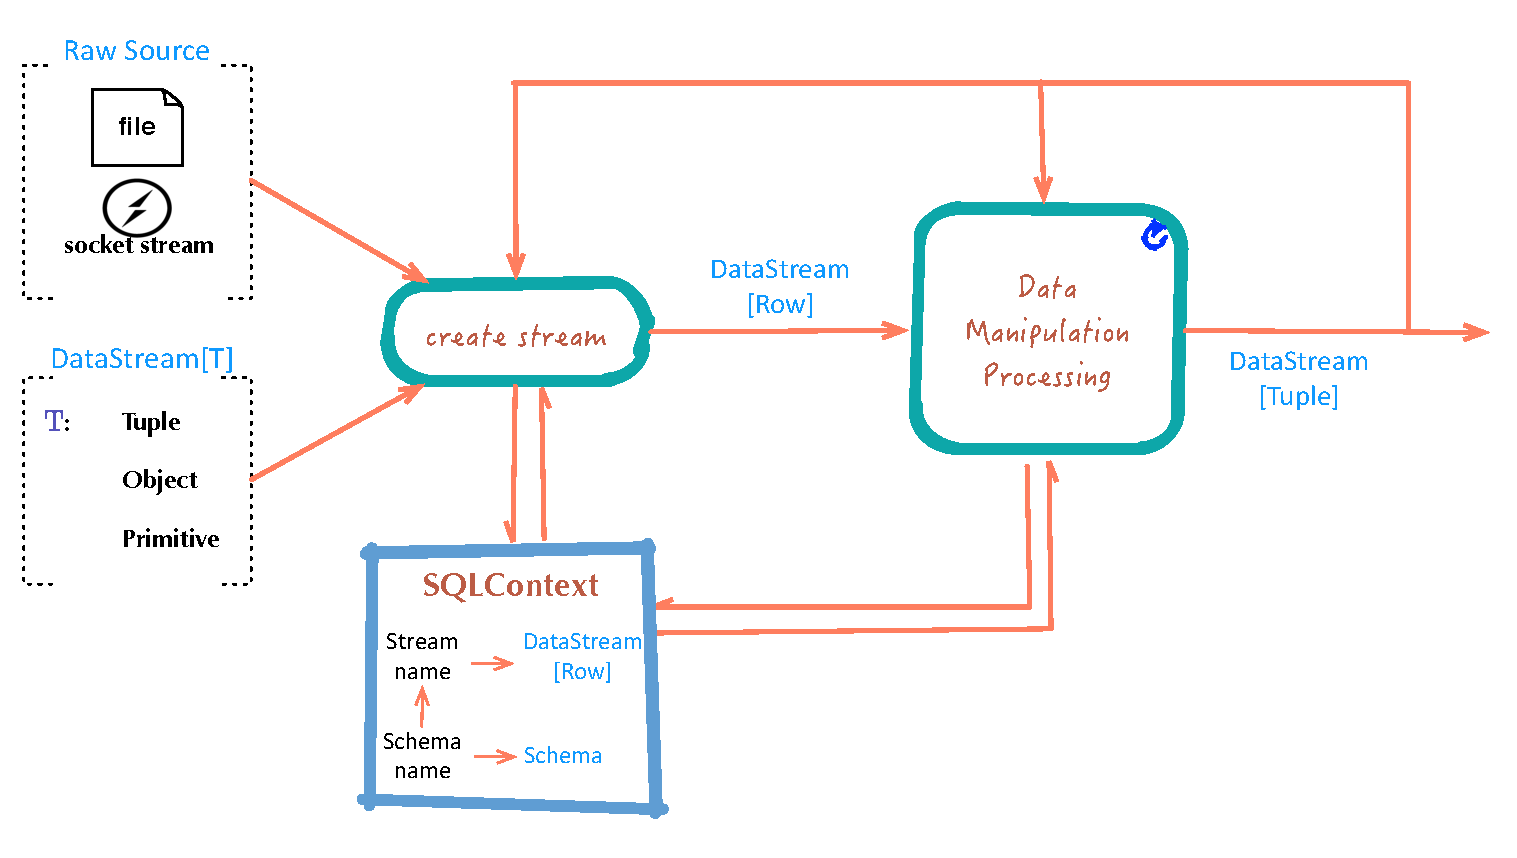
\includegraphics[width=1\textwidth]{Architecture}
\caption{Architecture}
\label{fig:Architecture}
\end{figure}


Figure~\ref{fig:Architecture} depicts the overall architecture of FlinkCQL query processing layer. It accepts data streams, query string and SQLContext as inputs and return one or more output data streams.
\subsection{Input Sources}
The query processing layer can connect to and process data streams from different data sources like file sources, web sockets, message queues (Apache Kafka, RabbitMQ, Twitter Streaming API …), and also from any user defined data sources. We classify the sources into 2 categories: \textit{Raw source} and predefined \textit{DataStream[T]} with \textit{T} is the type of stream elements.

\subsubsection*{Raw Source}


\textbf{Text file stream}: the source stream contains the lines of the files created (or modified) in a given directory. The system continuously monitors the given path, and processes any new files or modifications. The file will be read with the system’s default character set. FlinkCQL expresses the text file stream source via ``SOURCE FILE ( \textit{filePath, delimiter})'', the default delimiter is a comma. The delimiter is used to tokenize string and convert its result into tuples according to its schema


\textbf{Socket text stream}: the source stream contains the strings received from the given socket. Strings are decoded by the system’s default character set. Socket text stream is specified in FlinkCQL as ``SOURCE SOCKET ( \textit{filePath, delimiter})''
The user can optionally set a delimiter for the same purpose as in Text file stream.


\textbf{Message queue connectors:} There are pre-implemented connectors for a number of popular message queue services. Connectors provide an interface for accessing data from various third party sources (message queues). Currently three connectors are natively supported, namely Apache Kafka, RabbitMQ and the Twitter Streaming API. In the recent prototype of FlinkCQL, we have not designed any syntax for those connectors due to lacking of testing facilities. However, in the next prototype, we could extend its syntax at ease.

\subsection*{DataStream[T]}
The \textit{DataStream[T]} is the basic data abstraction provided by Flink Streaming. It represents a continuous, parallel, immutable stream of data of a certain type \textit{T}. Type \textit{T} could be :
\begin{itemize}
\item Primitive data type: integer, double, ...
\item Tuple type: which is a composite of multiple primitive data types such as \textit{(integer, string, integer)}
\item Class object: such as the instances of class \textit{CarEvent(id: Int, speed: Int)}
\end{itemize} 

\subsection{SQL Context} 

At the beginning, we encounter a problem of diverse data types of stream elements. A source stream can contains elements of string type (as in raw source), other primitive types, tuple or class instance. It is cumbersome and impractical to provide query processing for all kinds of source streams respectively. Thus, when a data stream is entitled to a schema (via \textit{Create Stream} or \textit{Insert} statement), we first transform the origin source stream to a Data Stream of a universal type \textit{Row} . \textit{Row} is simply a tuple containing \textit{an array of any data} including \textit{Null}. We do not specify the type of elements inside the Row. Those types will be derived from Schema.

Recall the example in ~\ref{query:createStream} to create schema and stream of ``StockTick''.
\begin{lstlisting}
	CREATE SCHEMA StockTickSchema (symbol String, sourceTimestamp Long, price Double, quantity Int, exchange String)
\end{lstlisting}

\begin{lstlisting} 
	CREATE STREAM StockTick StockTickSchema 
	SOURCE SOCKET ("98.138.253.109", 2000)
\end{lstlisting}

``StockTick'' is the Stream used inside FlinkCQL query. It is entitled to ``StockTickSchema'' and mapped to a real \textit{DataStream[Row]} which is derived from the socket text stream. The correlation between Stream and Schema is expressed in Figure~\ref{fig:SQLContext}. Be aware that the concept of Stream in FlinkSQL and DataStream in Flink is not identical. In fact, a Stream in FlinkSQL is a name to represent a \textit{DataStream[T]} in Flink.

All Stream-Schema-DataStream relationships are stored in 3 dictionaries of \textit{SQLContext}~(Figure~\ref{fig:Architecture}). 
Stream and Schema are unique but many Stream can share a Schema. And a Stream is mapped to a DataStream[T]. When users send out some further queries, query processing framework will lookup \textit{SQLContext} to decide which Stream-Schema is specified to generate an precise snippet of code.

\begin{figure}[h!] 
\centering    
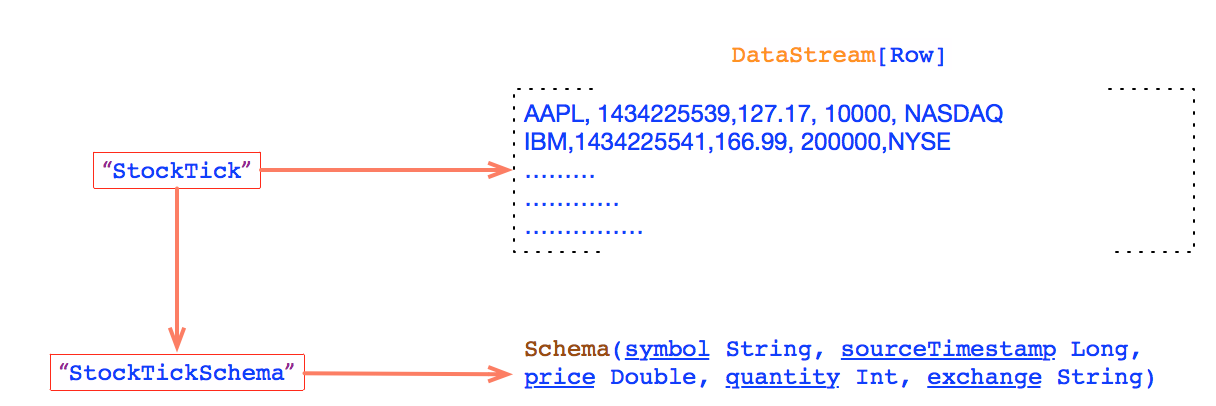
\includegraphics[width=0.8\textwidth]{SQLContext}
\caption{\textit{Stream}-\textit{Schema} mapping in \textit{SQLContext}}
\label{fig:SQLContext}
\end{figure}

\subsection{Data Manipulation Processing}
Data Manipulation Processing is used to process Data Manipulation Queries such as \textit{SELECT, MERGE, SPLIT, INSERT}. These queries specify which operators to process on given Streams and its Fields. First, system will first look up its SQLContext to retrieve the actual input \textit{DataStream[Row]} according to the Streams. Second, Operators and Schemas are together to decide how to transform input DataStreams to a new one. The output of processing is either one or more Streams which are updated into SQLContext or a DataStream of tuple. This DataStream of tuple can be consumed to create other Stream via \textit{CREATE STREAM} query. For examples, the output of \textit{SELECT} query is a DataStream of tuple but the outputs of \textit{SPLIT} query are more than one Stream~(along with its Schema and DataStream[Row]).

\section{FlinkCQL Query Interpreter}
\begin{figure}[h!] 
\centering    
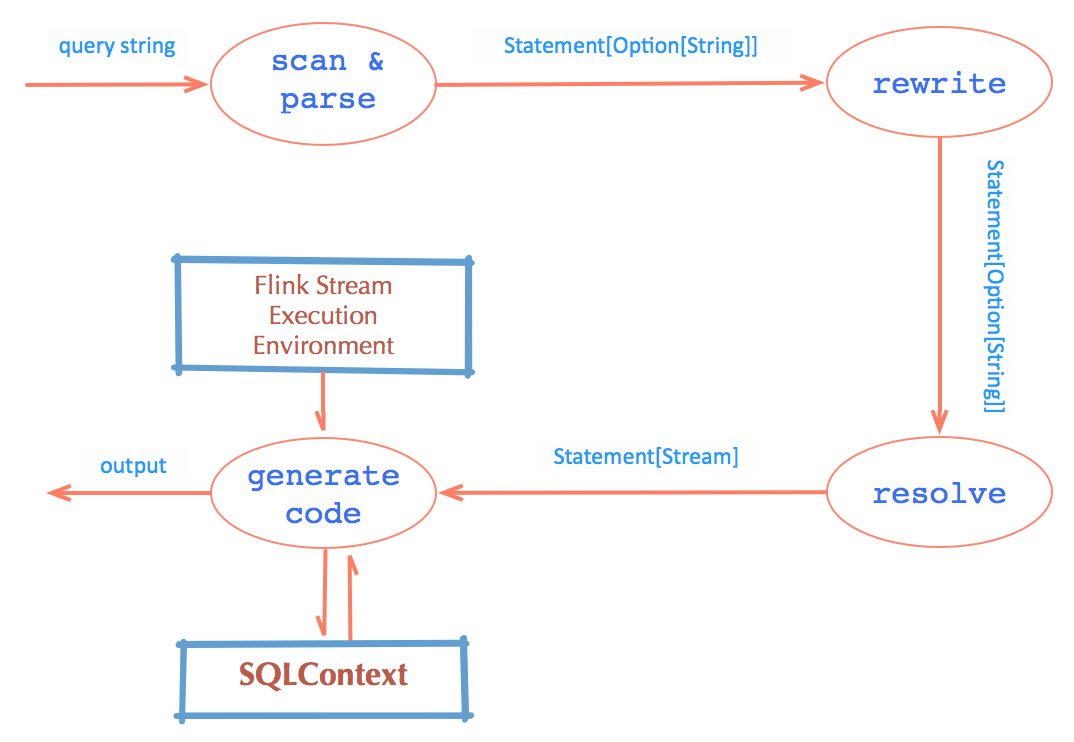
\includegraphics[width=0.7\textwidth]{QueryProcessing}
\caption{Query Processing}
\label{fig:QueryProcessing}
\end{figure}


Flink Stream Processing is offering a rich set of API to deal with one or  multiple input DataStream[T]. Our goal is to build an extension which accepts FlinkCQL query strings as commands and translate the commands to  corresponding programs constructed with Flink's APIs. Thus we are simply required to build a interpreter instead of a compiler from scratch. For this purpose, I have implemented a tree-based interpreter~\citep{Parr:2009} to process FlinkCQL queries. The idea is that the query interpreter executes program by constructing an abstract syntax tree~(AST) from the input query string and walking through the tree to generate a executable Flink program. More specifically, AST is a form of intermediate representation of the hierarchical syntactical structure of the source program written in query.  
	

The interpretation proceed through a series of well-defined phrases (Figure~\ref{fig:QueryProcessing}). Each phrase transforms or extracts information of use from the output of previous phrase and return a result which is a input of next phrase. In first proof-of-concept prototype, we build a pipeline consisting of 4 steps:
\begin{itemize}
	\item \textbf{Scanning and parsing:} serve to recognize the structure of the program, without regard to its meaning. This steps produce an AST with its root is highest semantic level of query : \textit{Statement[Option[String]]}

	\item \textbf{Rewriting} is to modify a sub-tree of AST to a more compact, optimal AST without changing the semantic of program.
	
	\item \textbf{Resolving:} It is possible that two or more streams, which are specified in query,  shares the same Schema. Thus, there is a potential ambiguity between two fields which have a identical name but belong to different stream. This phrase is to figure out to which fields refers. It is clear that we cannot generate code from an ambiguous AST.
	
	\item \textbf{Code generation}: In addition to a compact and unambiguous AST, the interpreter also lookup Stream-Schema information from SQLContext to generate a Flink program based on pre-defined translation rules. Last but not at least, we need the Flink stream execution environment to execute our generated code.
	
I describe all phrases processing a simple query: 
\begin{lstlisting}
	SELECT s.Quantity * Price, StockTick.Symbol 
	FROM StockTick AS s
\end{lstlisting}

\end{itemize}
\subsection{Scanning and Parsing}



This phrase is composed of 2 smaller steps : Scanning (lexical analysis) and parsing (syntax analysis).

\textbf{Scanner} reads characters from the query input and use regex patterns to groups them into \textit{lexemes}, which are the lexically meaningful units of the program, and produces as output tokens representing these lexemes. A token consists of two components: a token class and value. For example, in token \textit{<keyword, ``select">}, its class is \textit{keyword} and its value is ``select''. 

In FlinkCQL, we utilize several token classes which described in Table~\ref{table:TokenClass}


\begin{table}[h]
\caption{Token classes}
\centering
\label{table:TokenClass}
\setlength\extrarowheight{5pt}
\begin{tabular}{||>{\centering\bfseries}m{2in}   |>{\centering\arraybackslash}m{3in}||}
\hline
\textbf{Token class} & \textbf{Description} \\ \hline\hline
                 Identifier  & strings of letters or digits, starting with a letter. Regex: 
                                \\ \hline
                   Keyword	  & reserved keywords which cannot be declared as an Identifier. Example: select, from , as, insert, create, stream, schema,... \\ \hline
                   Integer		& a non-empty string of digits with sign (optional) \\ \hline %-?\d+
				   DecimalNumber		&  An integer followed by a decimal point and fractional part. One of the parts can be missing except for the decimal point. Example: $2.2$, $3.$, $.1$   \\ \hline %\textrm{(\d+(\.\d*)?|\d*\.\d+)}
					floatingPointNumber	& represented approximately to a fixed number of significant digits (the significand) and scaled using an exponent. For example, $3E-5$			               \\ \hline		%-?(\d+(\.\d*)?|\d*\.\d+)([eE][+-]?\d+)?[fFdD]?						
					stringLiteral		& Single quotes enclosing a sequence of string. For example: 'IBM', 'AAPL'			 \\ \hline
					Whitespace		& a non-empty sequence of blanks, newlines, and tabs.	 		                      \\ \hline								
					Other	& addition strings to make up the query. For example: (, ), . , {, }		                     \\ \hline							           							           							           							           
\end{tabular}
\end{table}

The regex pattern of these tokens are supported in \textit{JavaTokenParsers} class in Scala language. The output of this steps is a sequence of tokens. For examples, the list of tokens derived from the previous query sample (ignoring all Whitespace tokens):
\begin{lstlisting}
	<keyword, "SELECT">, <identifier, "s">, <other, ".">,
	<identifier, "Quantity">, <other, "*">, 
	<identifier, "Price">, <other, ",">, 
	<identifier, "StockTick">, <other, ".">,
	<identifier, "Symbol">, <keywork, "FROM">,
	<identifier, "StockTick">, <keywork, "AS">, 
	<identifier, "s">   
\end{lstlisting}

Oviously, scanner helps reduce the size of the input (there are many more characters than tokens) and remove extraneous characters like white space. Thus  , scanning is considered a pre-processing step to simplify the task of the parser.

\textbf{Parser} helps organize the input tokens into an AST. We build up an AST for each query using Packrat Parser which is available in Scala Parser Combinators. 
In short, Packrat Parsing is a technique for implementing backtracking,recursive-descent parsers, with the advantage that it guarantees unlimited lookahead and a \textit{linear} parse time. Using this technique, left recursive grammars can also be accepted.

To produce a complete meaningful AST using Scala parser combinators, we goes through a procedure of 4 substeps:
\begin{itemize}

\item \textbf{Step 1:} Executing the grammar

Based on the EBNF grammars of FlinkCQL which are described mostly in session~\ref{language}, we write equivalent executable grammars in Scala syntax with helps of combinators:
\begin{itemize}
	\item $p_1 \sim p_2$: sequencing combinator: must match $p_1$ followed by $p_2$. For example, \textit{Projection} clause is followed by \textit{From} clause
	\item $p_1$ | $p_2$: alternation combinator: must match either $p_1$ or $p_2$, with preference given to $p_1$. For example, window policy can be either time-based or count-based.
	\item $opt(p_1)$ : optionality combinator: may match $p_1$ or not. For example, \textit{Where} clause is optional in \textit{Select} statement.
	\item $rep(p_1)$ : repetition combinator: matches any number of repetitions of $p_1$. For instance: there is one or more entries in \textit{Projection} clause.
\end{itemize} 

In our processor, we define a grammar for \textit{Select} statement as :
\begin{lstlisting}
lazy val selectStmtSyntax = projectionClause ~ fromClause ~ opt(whereClause) ~ opt(groupByClause)
\end{lstlisting}
It means that \textit{projectionClause} is followed by a \textit{fromClause}, an optional \textit{whereClause} and a optional \textit{groupByClause} in order.

The topmost abstraction of the FlinkCQL grammar is \textit{Statement}. It can express either \textit{Select}, \textit{Create schema}, \textit{Create stream}, \textit{Merge}, \textit{Insert}, \textit{Split} query syntax.
\begin{lstlisting}
lazy val stmt = (selectStmtSyntax| createSchemaStmtSyntax | createStreamStmtSyntax | MergeStmtSyntax  | insertStmtSyntax| splitStmtSyntax)
\end{lstlisting}

The parsing process of the grammar will generate a parse tree but the ouput tree is represented by a string. Let us consider the parse tree of the sample query:
\begin{lstlisting}
((List(((((s~.)~Quantity),*,Price)~None),(((StockTick~.)~Symbol)~None))~(((StockTick~None)~Some(s))~None))~None)~None
\end{lstlisting}
The List denote that the query require 2 entries in projection clause. The last 2 \textit{None} values express that \textit{Where} clause and \textit{GroupBy} clause is missing.

However, this output format is useless for next steps since it is also a string in a different way. Thus, we need to design a more powerful abstract semantic model and integrate it to the parser tree so that the parser will return a \textbf{Statement} object , instead of a string. Once we obtain a \textbf{Statement} object, we are able to exploit its components recursively for further traversal. As long as we build a complete semantic model for FlinkCQL (in Step 2), Scala offers a bunch of function application combinators to plug directly these semantic abstractions to the parse rules (in Step 3)

\item \textbf{Step 2:} Building the semantic model for the FlinkCQL

As we mentioned above, the topmost abstraction of FlinkCQL is \textit{Statement} which we can defined in Scalas as a \textit{trait} (similar to Interface).
\begin{lstlisting}
	sealed trait Statement[T]
	case class CreateSchema[T](...) extends Statement[T]
	case class CreateStream[T](...) extends Statement[T]
	case class Select[T](...) extends Statement[T]
	case class Insert[T](...) extends Statement[T]
	case class Merge[T](...) extends Statement[T]
	case class Split[T](...) extends Statement[T]
\end{lstlisting}

Each inherited class of \textit{Statement} contain its attributes as child nodes in the whole AST model. Each of these attribute may contains several child notes as well. For example, each \textit{Entry} in Select's projection clause is composed of its name, alias name and an expression

\begin{lstlisting}
	case class Entry[T](name: String, alias: Option[String], expr: Expr[T])
\end{lstlisting}

We are then able to access to this \textit{Entry}'s expression \textit{expr}. Hence, we are able to build up a complete semantic model for FlinkCQL using a top-down approach.

\item \textbf{Step 3:} Generating the AST using function application combinators.

Up to now, we have a set of parser rules which produce a parser tree, and also design a underlying domain-level abstractions of FlinkCQL. The last step to generate a AST is to plug suitable abstractions into grammar rules using Scala function application combinators. Consider the following examples of \textit{Select} query:

\begin{lstlisting}
	lazy val selectStmtSyntax = 
	selectClause ~ fromClause ~ opt(whereClause) ~opt(groupBy) ^^ {
    case s ~ f ~ w ~ g => Select(s, f,w, g)
  }
\end{lstlisting}

We do use the combinator ``$\wedge \wedge$'' to deconstruct the tuple returned by the parser and to thread it into the anonymous pattern-matching function. The last result is a Select object as above. Similar integration rules are applied for other parsing components across the process. 
If the whole parsing process is successful, the processor effectively built the whole semantic model as the AST used by next phrase.

For the sample query, this step return a AST with topmost abstraction is a Select object which is visualized in Figure~\ref{fig:Parse}

\begin{lstlisting}
	Select(List(Entry(<constant>,None,ArithExpr(ArithExpr(Field(Quantity,Some(s)),*,Field(Price,None)),+,Constant((Double,Double),10.2,double))), Entry(Symbol,None,Field(Symbol,Some(StockTick)))),ConcreteStream(Stream(StockTick,Some(s),false),None,None),None,None)
\end{lstlisting}
 

\end{itemize}


\begin{figure}[h!] 
\centering    
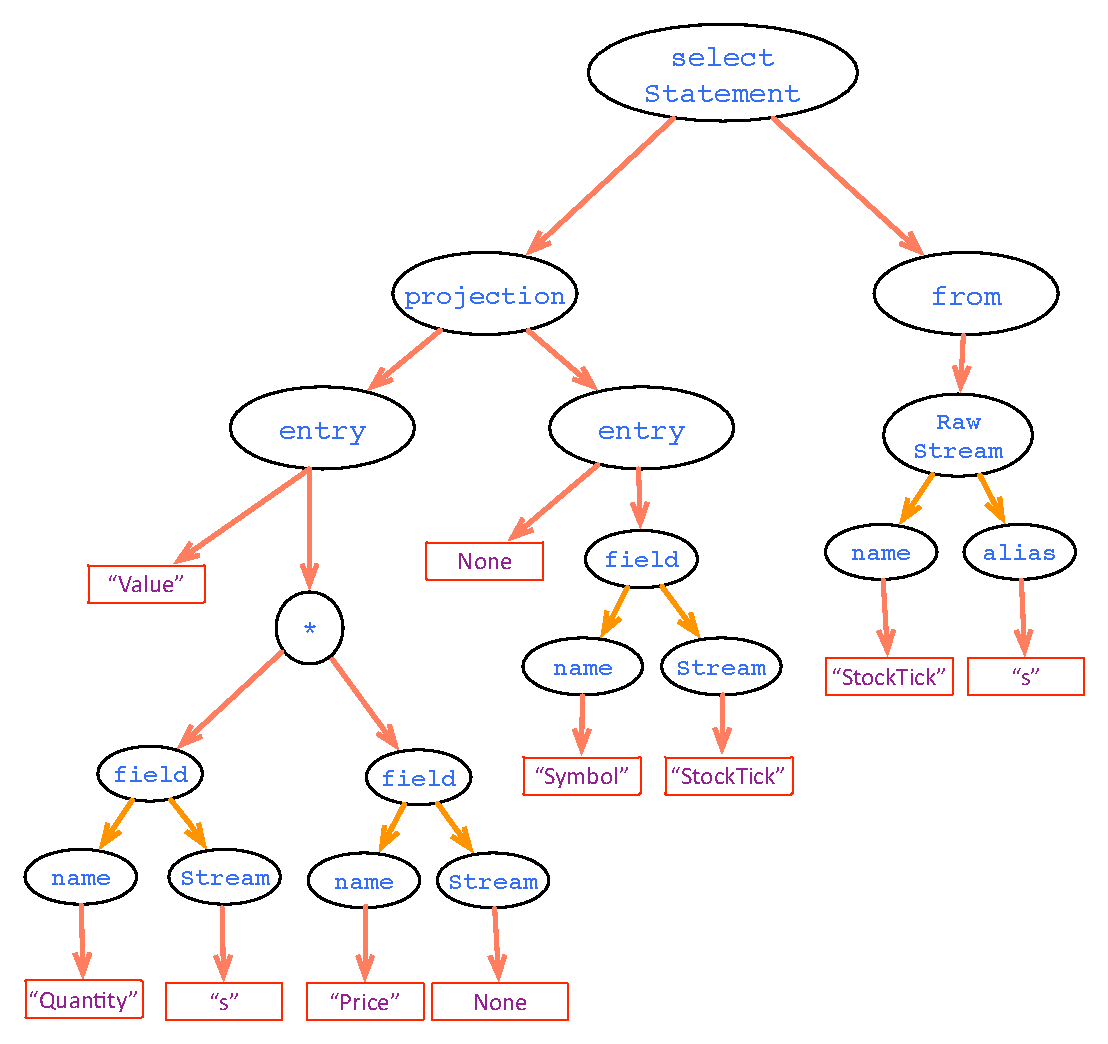
\includegraphics[width=0.7\textwidth]{Parse}
\caption{Parse}
\label{fig:Parse}
\end{figure}


\subsection{Query Rewriting}
The AST, which is produced from previous phrase, is analyzed directly from FlinkCQL query string. For some reason, the query may not be optimal. Consider a very simple example, one entry in projection clause: $Quantity\, +\, Quantity$, which could be replaced by $Quantity\, *\, 2$. Such query rewriting rules optimize the AST but optional. 

We  do implement a AST rewriting rule that helps to reduce the numbers of translation rules in Code Generation phrase. This rewriting rule is apply to a subquery clause which produce an output \textit{Windowed Stream}. If we able to rewrite it to a new subquery that returns a concrete DataStream instead, we need not to define any translation rule for Windowed Stream anymore.

Consider two queries which have identical meaning:

\begin{lstlisting}
From (select Symbol,Price From StockTick [Size 3]) as s
=
From (select Symbol,Price From StockTick) [Size 3] as s
\end{lstlisting}

In the first query , its subquery will return a Windowed Stream which is not supported. Therefore the query is invalid. In the second query, its subquery return a concrete DataStream which is acceptable.

The change we made on AST structure of the first query is to move the window of the subquery to its upper-level (From clause). Thus,in the new structure (query 2), the subquery will produce a \textit{DataStream} of \textit{(Symbol, Price)} whereas the upper-level will process on a windowed stream with size of 3. 

\subsection{Resolving}
Looked at the Figure~\ref{fig:QueryProcessing} again,  the output of last 2 phrases is a \textit{Statement} object with type parameter is \textit{Optional[String]}.
It indicates that there are some potential fields/columns whose streams are not specified in AST. In other words, the value of \textit{stream} is None.
\begin{lstlisting}
	case class Field[T](name: String, stream : T)
\end{lstlisting}

In the example (Figure~\ref{fig:Parse}), there are three fields: ``StockTick.Symbol”, ``s.Quantity”, ``Price”. Their \textit{stream} value is ``StockTick", ``s" , and \textit{None} respectively. The interpreter is not sure if those identifiers of streams do exist or not. Moreover, it is impossible to operate on a field whose stream is ambiguous. Thus, we need to figure out  which streams that ``Symbol”, ``Quantity”, ``Price”  fields refer to.

This step helps to resolve the problem so that we can generate the exact Flink program in next phrase.

To solve the problem, each Statement maintains a list of its Streams so that FlinkCQL processor can look up to resolve which streams the fields refer to. Recall the example, processor acknowledges that there is one Stream exists whose name and alia are ``StockTick'' and ``s''. Since the prefix of the fields match either those values or \textit{None}, the stream of fields are updated to ``StockTick'' (Figure~\ref{fig:Resolve})

The output of this phrase is a rewritten AST as \textit{Statement[Stream]} since stream values of  fields are totally resolved.

\begin{lstlisting}
	Select(List(Entry(<constant>,None,ArithExpr(Field(Quantity,Stream(StockTick,Some(s),false)),*,Field(Price,Stream(StockTick,Some(s),false)))), Entry(Symbol,None,Field(Symbol,Stream(StockTick,Some(s),false)))),ConcreteStream(Stream(StockTick,Some(s),false),None,None),None,None)

\end{lstlisting}

\begin{figure}[h!] 
\centering    
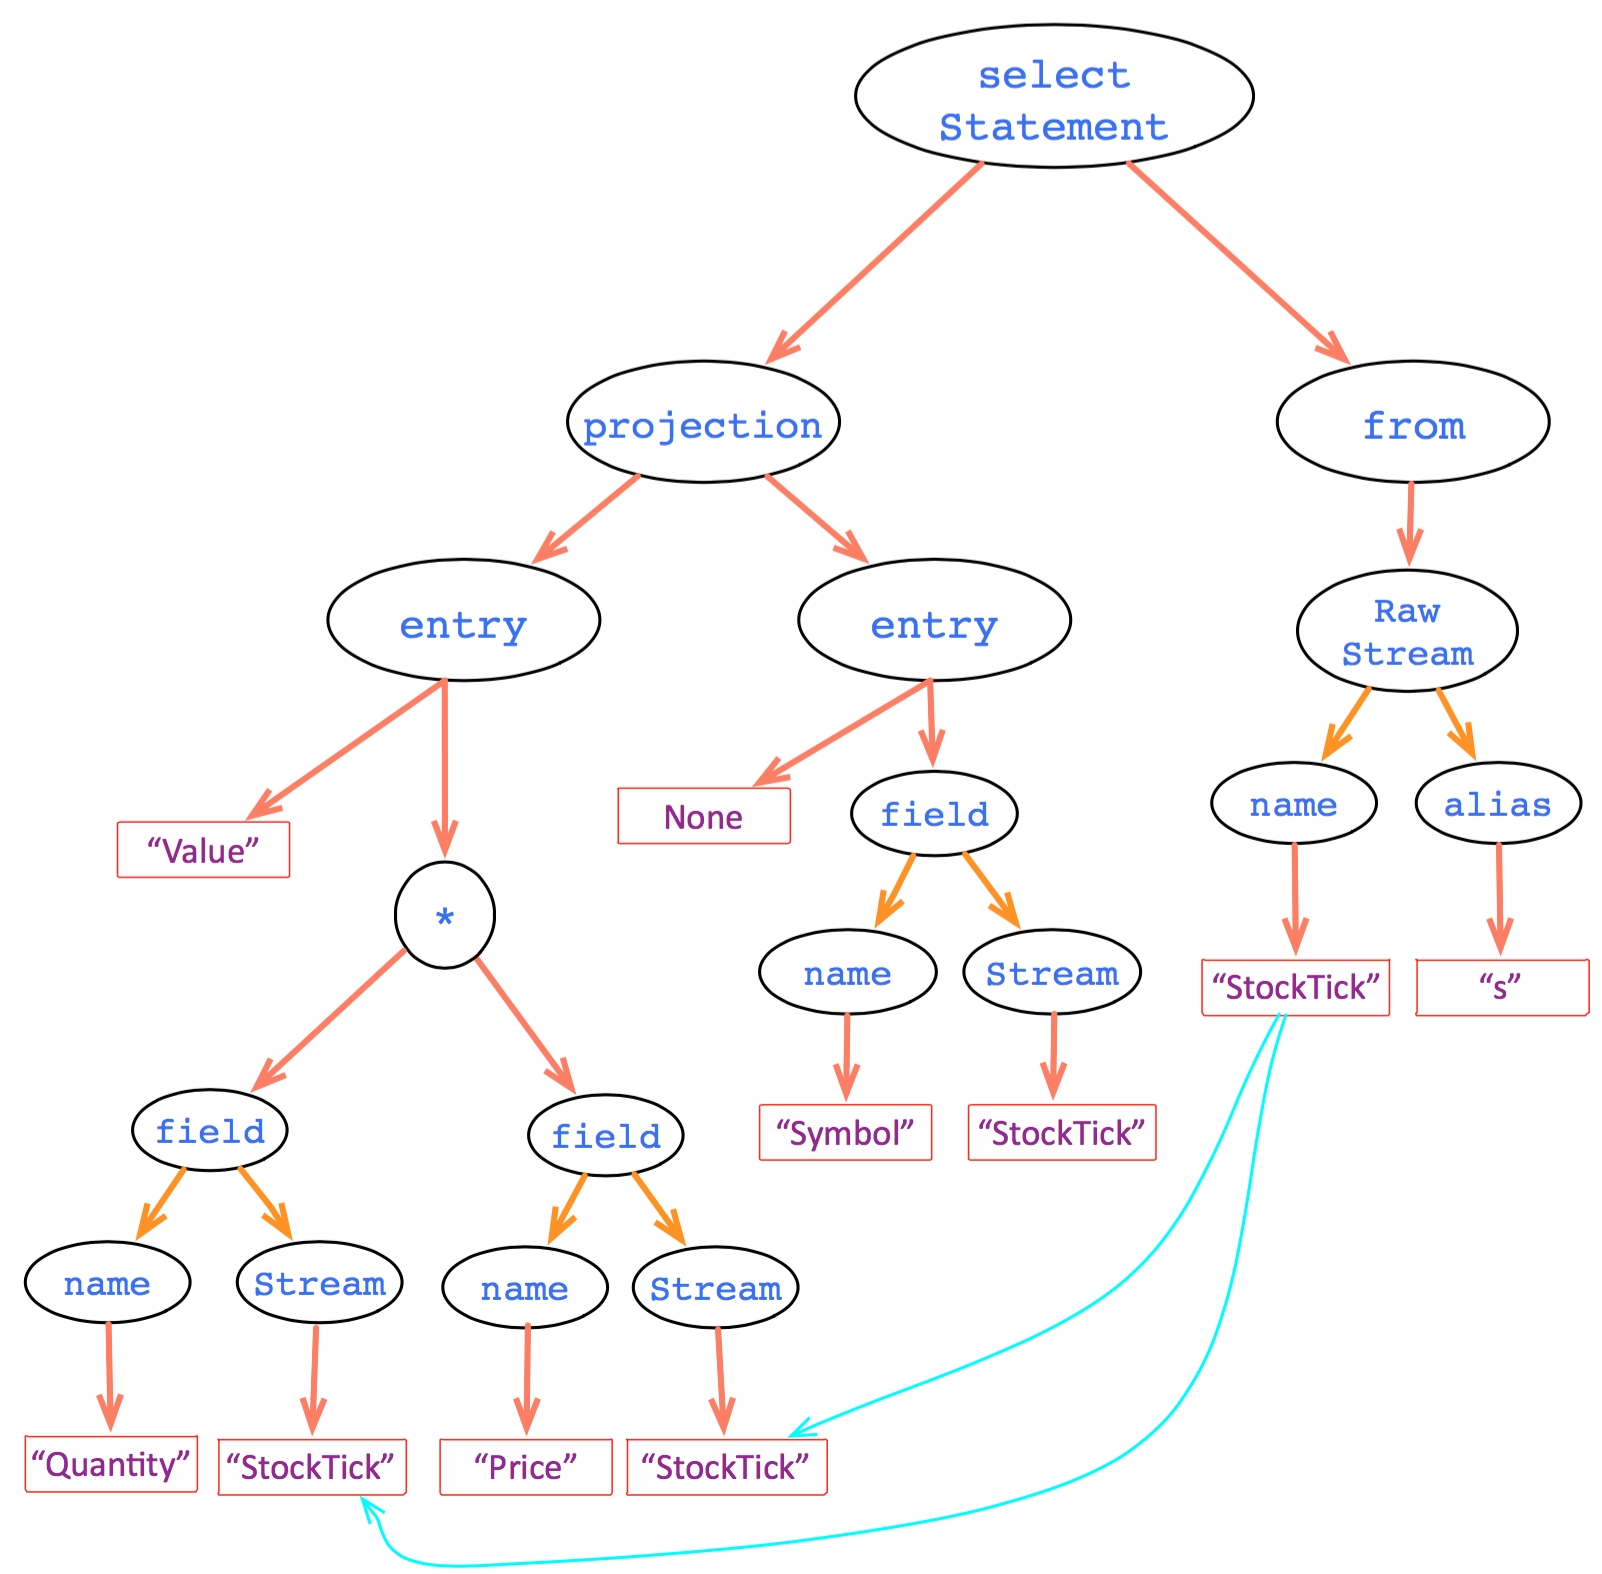
\includegraphics[width=0.7\textwidth]{Resolve}
\caption{Resolve}
\label{fig:Resolve}
\end{figure}


\subsection{Code Generation}
The last phrase of interpretation is to generate an executable Flink program in Scala from the output AST of previous phrase. Scala language provides compile-time and run-time reflection to build or manipulate a Scala Abstract Syntax Tree which used to represent Scala programs. 

The compile-time reflection is realized in the form of macros, which provide the ability to execute methods that manipulate Scala AST at compile-time. However, Scala also provide ToolBox api one can generate, compile Scala AST and run Scala code at runtime. 

I design a different set of translation rules to derive a Scala AST from different Statement object which serve as FlinkCQL AST. The Scala AST could be compiled to Flink executatble program in either compile-time or runtime.

Supposed that 
\begin{equation}
	\overline{X} = Generate(X)
\end{equation}
 with $X$ is object abstraction denoting a subtree of a AST and $\overline{X}$ is an equivalent block of Scala AST code generated from $X$

\subsubsection*{Select statement Generation}
Select object has 4 attributes: Projection \textit{proj}, StreamReference \textit{streamRef}, Where \textit{w} and GroupBy \textit{by}. \textit{Where} and \textit{Groupby} attribute object are optional. 

Supposed that Select object $s$ :
\begin{lstlisting}
s = Select (proj, streamRef, w, by)
\end{lstlisting}

StreamReference object has up to 3 attributes :  Stream \textit{stream}, window Specification \textit{ws} and Join \textit{j}.
\begin{lstlisting}
	streamRef = StreamReference(stream, ws, j)
\end{lstlisting}

However, we can generate a StreamReference object from Join object in condition that WindowSpecification object $w_1$ and $w_2$ specify a same time-based window. Otherwise, processor is not able to generate code of Join object due to Flink's functionality constraint.
\begin{equation}
	\textrm{j = StreamRef(}s_1,\, w_1,\, \textrm{Join(}s_2,\, w_2, \textrm{joinCondition))}
\end{equation}

\begin{equation}
StreamReference(stream, ws) = \overline{  s_1}\textrm{.join(}\overline{s_2})\textrm{.onWindow(}\overline{s_2}\textrm{).where(}\overline{joinCondition}\textrm{)}
\end{equation}
in which, ``join'', ``onWindow'', ``where'' are Flink's functions applied to  \textit{DataStream[Row]} object generated from $s_1$

Therefore, we could assume that
\begin{lstlisting}
	streamRef = StreamReference(stream, ws)
\end{lstlisting}

There are 2 possible scenarios for optional WindowSpecification object \textit{ws}:
\begin{enumerate}
	\item \textbf{\textit{ws} is undeclared}. It means that processor does query on a \textit{DataStream[Row]}.  The generated block of Flink code for Select object $s$ is defined as
	
	\begin{equation}
	\overline{s}\, =\,\overline{stream} .filter(\overline{w}).map(\overline{proj})
\end{equation}
	Be aware that \textit{GroupBy} operator is not applicable for a concrete Stream because it partitions the original data stream into multiple undefined streams which processor can not feed as input streams for other queries. 
	
	\item \textbf{\textit{ws} is defined} as:
		\begin{lstlisting} 
	ws = WindowSpecification(size, every, partitioned)
\end{lstlisting}
It means that processor does query on a \textit{DataStream[Row]} discretized by windowing technique. The generated block of Flink code for \textit{Select} object $s$ is defined as


\begin{multline}
	\overline{s}\, =\,\overline{stream} .filter(\overline{w}).groupBy(\overline{by}).map(\overline{proj})	.window(\overline{size}).every(\overline{every}) \\
	.groupBy(\overline{partitioned}).mapWindow(\overline{proj}).flatten
\end{multline} 


	
\end{enumerate}


\subsubsection*{Merge statement Generation}

\textit{Merge} object has only one member attribute which is the list of input \textit{Streams}
\begin{equation}
	\textrm{m = Merge(List(} s_1, s_2, ...s_k \textrm{))}
\end{equation}

The generated block of Flink code for \textit{Merge} object \textit{m} is:
\begin{equation}
	\overline{m} = \overline{s_1}\textrm{.merge(}\overline{s_2}, ...\overline{s_k} \textrm{))}
\end{equation}

\subsubsection*{Split statement Generation}

Split object $sp$ has 2 attributes: source stream $s$ and list $insertList$ of \textit{Insert} objects. Process first extracts targeted Streams and split conditions in \textit{Where} clause  of \textit{Insert} object. It then collects those information to a tuple list $tupleList$ of \textit{(Stream, Where)}. Finally, a Flink program is generated based on $tupleList$ list ,  stream $s$ and \textit{split} function in Flink API.

\begin{align}
	sp = Split(s, insertList)) \\
	tupleList: List(Stream, Where) = extract(insertList) \\
	\overline{sp} = \overline{s}\textrm{.split(}\overline{tupleList})
\end{align}

For other statements such as \textit{CreateSchema}, \textit{CreateStream} and \textit{Insert}, processor simply creates new objects, establish mapping between Stream and Schema. At the end, all of mapping relationship will be updated to \textit{SQLContext} for later use.

\section{Evaluations}
\subsection*{Experimental environment}
The proof-of-concept prototype of FlinkCQL query interpreter is built and tested on a machine equipped Intel Core i7 2,6 GHz, memory of 16Gb RAM, and free space of 10Gb in harddisk, and running MacOS 10.10.3.

The source code is committed to Flink repository at Github~ (\href{https://goo.gl/V6Y5dK}{https://goo.gl/V6Y5dK})\footnote{\href{https://github.com/mbalassi/flink/tree/linq/flink-staging/flink-streaming/flink-streaming-DSL}{https://github.com/mbalassi/flink/tree/linq/flink-staging/flink-streaming/flink-streaming-DSL}}


\subsection{Two testing phrases}
Recall that processor goes through 4 phrases to complete the interpretation process. The first 3 phrases is to build up a semantic AST from a input query string. The last phrase is to generate an executable program from the AST,  \textit{SQLContext} and Flink streaming execution environment. We recognize the first 3 phrases is nearly independent from input data streams.  Therefore, we decide to evaluate the results in 2 phrases:

\begin{itemize}
	\item \textbf{AST construction} testing phrase: to evaluate the output AST of the first 3 steps: scanning -  parsing, rewriting and resolving.
	\item \textbf{Executable Program} testing phrase: to evaluate the complete interpretation process.
\end{itemize}

\subsubsection{Phrase 1: AST Construction}
Each Stream Processing engine may define its own continuous query language. Up to now, there is no benchmark such as \textit{TPC-H} to evaluate and measure the correctness and performance of query-based stream processing engines in general. 
Hence, we decide to test the AST construction on our own set of queries (Appendix A). Queries are broken into 6 groups corresponding to its types: 
\begin{itemize}
	\item Group 1: Create Schema queries
	\item Group 2: Create Stream queries
	\item Group 3: Select queries
	\item Group 4: Merge queries
	\item Group 5: Insert queries
	\item Group 6: Split queries
\end{itemize} 

\begin{figure}[h!] 
\centering    
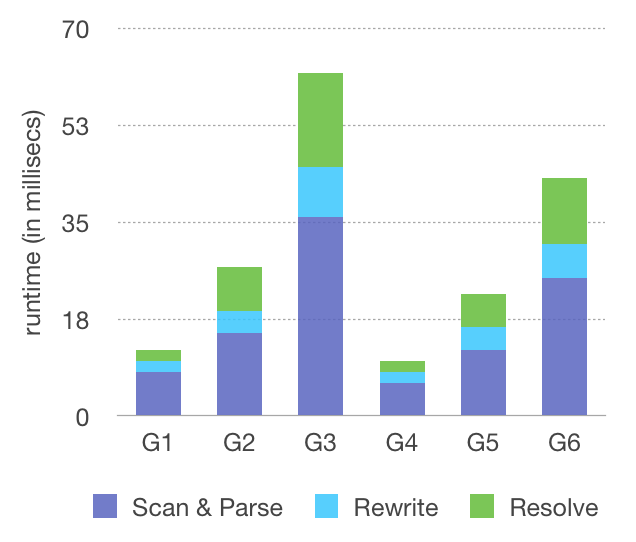
\includegraphics[width=0.6\textwidth]{ASTConstruction}
\caption{AST Construction Testing}
\label{fig:ASTConstruction}
\end{figure}

Figure~\ref{fig:ASTConstruction} depicts the \textit{maximum} runtime (in milliseconds) of each phrases in each group. We observe that Select and Split query usually take longer time to process since they have most complicated syntax. However, the maximum of total process is less than \textbf{70 milliseconds}  only. In additional, a large portion of time is to parsing the input query string to the first AST. 

\subsubsection{Phrase 2: Executable Program}



We finally implement a simple but complete application consisting of 4 queries in order:

\begin{table}[h!]
\caption{Code Generation Test}
\centering
\label{table:GenerationTest}
\setlength\extrarowheight{5pt}
\begin{tabular}{||>{\centering\bfseries}m{0.5in}|>{\centering\arraybackslash}m{5in}||}
\hline
\textbf{No} & \textbf{Query} \\ \hline\hline
     		1 & 	       create schema carSchema (carID Int, price Int)\\ \hline
     		2 & create stream CarStream carSchema source stream ('CarSales')	       \\ \hline
     	3 & 		select carID, c.price * 0.05 as tax from CarStream as c       \\ \hline
     	4 &	select c.pr * 1.05 as fullTax from (select pr from (select carID , price  as pr from CarStream) as d) as c	       \\ \hline
	           				
 \end{tabular}
\end{table}

We are able to register a \textit{CarStream} stream which is derived from user-defined \textit{DataStream[Car]} named ``CarSales''
\begin{lstlisting}
 	case class Car (carID: Int, price: Int)
\end{lstlisting}

The third query is to observe the tax which owners need to pay for their cars. The last query is just to demonstrate that we are able to write n-nested subquery with FlinkCQL. Even with this complex query, the whole interpretation process takes less than 60 milliseconds to generate an executable program since the query was received.  Consider that the stream is possibly unbound, the latency of 60 milliseconds to translate the query is not considerable. 

\begin{figure}[h!] 
\centering    
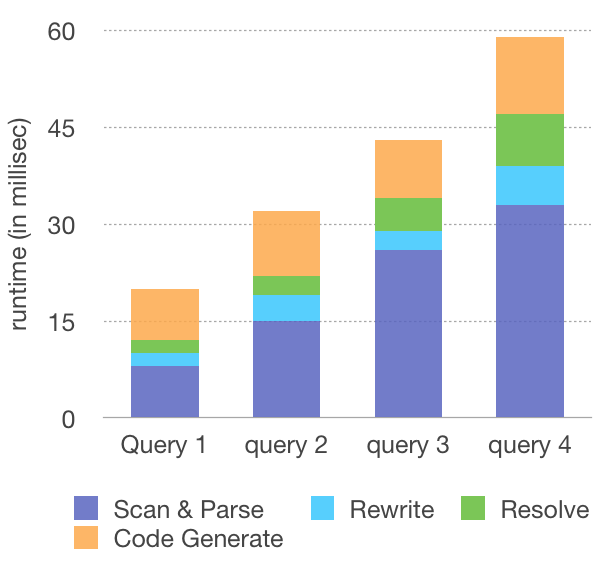
\includegraphics[width=0.6\textwidth]{ExecutableProgram}
\caption{Executable Program Testing}
\label{fig:ExecutableProgram}
\end{figure}

\section{Future Work}

Though we ran experiments successfully on our set of queries, the number of queries is till very restricted and objective. We are not able to test all possible queries with limited user-generated queries. Our future work is to build a Random Query Generator~(RQG) for coverage and functional testing. RQG generates thousands of random queries based on SQL templates the queries must conform to. The idea is that we build a Finite State Machine model from the templates and decide how to walk around, expand an AST and generate numerous valid queries  probabilistically. 

For the last phrases of Code Generation, we have employed Scala \textit{Macros} technique to gradually construct the Scala AST code which is executed at \textit{compile-time}. However, there is a disadvantage 
when applying Macro to generate Flink program. Some  Flink functions required informations extracted from SQLContext at runtime. For example, ``mapWindow'' function is applied on a \textit{WindowStream} to  transforms a window to other type of window. We able to use ``mapWindow'' to reduce the window to a tuple (using aggregation function) which may fulfil the projection clause of \textit{Select} query. However, the parameter of this function is a anonymous function which required  to specify its input type and output type. Although the output type could be deduced by AST and Schema in SQLContext, we are unable to extract a specific SQLContext information at compile-time. Thus, we could not generate code for ``mapWindow'' parameters. One of potential solution is to generate and execute code at runtime using \textit{ToolBox Api}. One can deduce the type of the output, plug it into Scala AST of mentioned anonymous function and generate this function at runtime. ``mapWindow'' may work in this case. 

In conclusion, we may use runtime compilation approach to generate the Scala AST. Moreover, a Random Query Generator is needed in the purpose of testing.

